\documentclass{article}
\usepackage{graphicx}
\usepackage{standalone}
\usepackage{multicol}
\usepackage[parfill]{parskip}

% Used for sequence diagram
\usepackage{pgf-umlsd}
\usepackage{tikz}
\usetikzlibrary{shapes,arrows}

%used for subsubsubsections
\setcounter{tocdepth}{5}
\setcounter{secnumdepth}{5}

\usepackage{changepage}   % for the adjustwidth environment

% syntax highlighting
\usepackage{listings} 
\usepackage{color}
\definecolor{lightgray}{rgb}{.9,.9,.9}
\definecolor{darkgray}{rgb}{.4,.4,.4}
\definecolor{purple}{rgb}{0.65, 0.12, 0.82}
\definecolor{codegreen}{rgb}{0,0.6,0}
\definecolor{codegray}{rgb}{0.5,0.5,0.5}
\definecolor{codepurple}{rgb}{0.58,0,0.82}
\definecolor{backcolour}{rgb}{0.95,0.95,0.92}
\lstdefinelanguage{JavaScript}{
  keywords={typeof, new, true, false, catch, function, return, null, catch, switch, var, if, in, while, do, else, case, break},
  keywordstyle=\color{blue}\bfseries,
  ndkeywords={class, export, boolean, throw, implements, import, this},
  ndkeywordstyle=\color{darkgray}\bfseries,
  identifierstyle=\color{black},
  sensitive=false,
  comment=[l]{//},
  morecomment=[s]{/*}{*/},
  commentstyle=\color{purple}\ttfamily,
  stringstyle=\color{red}\ttfamily,
  morestring=[b]',
  morestring=[b]"
}

\lstset{
   language=JavaScript,
   backgroundcolor=\color{lightgray},
   extendedchars=true,
   basicstyle=\footnotesize\ttfamily,
   showstringspaces=false,
   showspaces=false,
   numbers=left,
   numberstyle=\footnotesize,
   numbersep=9pt,
   tabsize=2,
   breaklines=true,
   showtabs=false,
   captionpos=b
}

% Hyperlinks
\usepackage[colorlinks,allcolors=blue]{hyperref}
\usepackage[normalem]{ulem}
\usepackage{xcolor}
\makeatletter
\begingroup
  \catcode`\$=6 %
  \catcode`\#=12 %
  \gdef\href@split$1#$2#$3\\$4{%
    \hyper@@link{$1}{$2}{\uline{$4}}% or \underline
    \endgroup
  }%
\endgroup
%Used for bibliography
\usepackage[british]{babel}
\usepackage[%
  autolang=other,
  backend=bibtex      % biber or bibtex
%,style=authoryear    % Alphabeticalsch
 ,style=numeric-comp  % numerical-compressed
 ,sorting=none        % no sorting
 ,sortcites=true      % some other example options ...
 ,block=none
 ,indexing=false
 ,citereset=none
 ,isbn=true
 ,url=true
 ,doi=true            % prints doi
 ,natbib=true         % if you need natbib functions
]{biblatex}
\addbibresource{../Bibliography/Bibliography}

\begin{document}
    \section{Design}
    
    \subsection{Overview}
    
In this paper, I present an ``end-to-end verifiable system'' built on the Ethereum Blockchain, i.e., a system where a voter can be assured their vote has been fairly counted, only eligible voters are allowed to vote and the tallied results of the election are publicly verifiable.

Although this system has been designed and developed with the idea of a national general election in mind, the protocols and ideas involved could be applied to smaller scale ballots which wish to provide transparency in their audit. Although we wish to minimize trust in a central authority, due to the nature of these type of elections (where there needs to be some degree of voter eligibility verification), we cannot fully decentralize this system as we need to only allow those eligible the rights to vote. Despite needing to verify an individual we still need to ensure that their votes are publicly anonymous, especially given the public transactions underpinning the blockchain concept while providing the ability for an individual to verify that their vote was correctly counted.

I do not see this system as a direct ``replace all'' for national election voting. I believe there will still be a need for traditional voting implementations in certain situations; for example, maintaining postal vote for the elderly who may not have the technical capability or equipment for online voting. However I do think that this could be phased in along side traditional voting, eventually replacing the pre-existing e-voting systems and ultimately becoming the main way for the majority of people to choose their government. 

The designed schema for this protocol is the following:
\begin{enumerate}

\item Ballot creation:
	\begin{itemize}
		\item The available ballots in the election are designed and decided upon.
		\item A smart contract is created and pushed to the blockchain for each ballot containing all of the voting options.
	\end{itemize}

\item Pre-election voter verification:
	\begin{itemize}
		\item Voter registers with an external voter registrar after providing a valid ID (this could be accomplished using pre-existing government electoral registration protocols).
		\item This external registrar generates a \textit{user\_id} and \textit{nonce} which can be used by the voter to log in to the system.
		\item This \textit{user\_id} is then tied to any ballots the voter is eligible for.
	\end{itemize}
	
\item Voter registration:
	\begin{itemize}
		\item The voter logs into the system using the received \textit{user\_id} and nonce upon which time they are immediately required to change their login credentials.
		\item The voter can then register to vote through the online system for each of the ballots they are eligible for.
		\item A unique Ethereum address, \textit{voter\_address}, is generated and validated (while not being linked to the \textit{user\_id})
		\item The \textit{user\_address} is added to the ballots smart contract which entitles this address to vote in that ballot.
		\item The address is funded with enough Ether for the voter to cast their vote.
	\end{itemize}

\item Voting:
	\begin{itemize}
		\item When the voter decides to cast their vote they are presented with an interface mirroring the options in the ballot smart contract.
		\item Upon the voter selecting their options the contract is funded with the voters selected options.
		\item At this point the voters choice is immutably entered into the blockchain and the tally is verifiable by all.
	\end{itemize}

\item Election result:
	\begin{itemize}
		\item Once the election is over, due to the nature of the smart contract design, no more votes can be added for any candidate.
		\item The tally for each candidate is publicly verifiable by anyone along with all of the funded transactions casting votes.
	\end{itemize}

\end{enumerate}

\cleardoublepage    
\subsection{Docker}
Over the past few years, container technology has become increasingly promising as a means to seamlessly make software available across a wider range of platforms \& allow developers to worry less about the eventual runtime environment (as this can be standardized). Docker containers provide a way to ``wrap up a piece of software in a complete filesystem that contains everything it needs to run'' \citep{51_kowalkowski_2017}.

There are several benefits to the use of Docker containers; This could substantially reduce the effort required to create and validate a new software releases, since docker containers create their own dedicated environment, testing on one OS means that the application will run the same on any OS capable of running Docker. In addition, docker containers provide a quick and easy way to install and use a software release, for our application this could mean faster patches if needed as you would simply need to swap out the docker image being used. Other benefits include faster bootup of containers (compared to just virtualization), closer development to production parity, immutable infrastructure and improved scaling (on a per-container basis) \citep{52_scherensstraat_2017}. There is also a security argument to be made for using containers, as they offer a degree of isolation for each enclosed application and only expose those services which you decide. The previous point about patching also add to security, as legacy applications often forgo patches in sensitive environments due to the possibility of breakages. When using containers, changes can be fully tested in the container which can then be swapped into the production environment \citep{53_security_risks_and_benefits_of_docker_application_containers_2017}.

All of my development for this project was conducted inside of Docker containers. I decided on this because there are very distinct separations between the applications which make up my system (this is described in the section on \hyperref[sec:SystemDesign]{System Design \ref*{sec:SystemDesign}}), so running each one inside a docker container seemed the logical thing to do. It also meant that I could control the startup of the system as a whole \& expose (between containers) only those services necessary to communicate.

\cleardoublepage    
\subsection{Internal node networking}
\label{sec:InternalNodeNetworking}
The design of the system requires services to be split up into separate nodes each with a specific set of functionalities. Many of these nodes require services from other nodes to operate (for example, the ``Application Sserver'' querying the ``Ballot Regulator'' for the list of ballots available to a user) and so efficient inter-node communication is vital. I ultimately decided to use the Python networking toolkit Twisted \citep{63_twisted_2017} for all of the networking of this system. The main draw of Twisted was that it offers asynchronous messaging through its AMP protocol.


I chose to use asynchronous messaging for a few reasons. First, is that ultimately there will be a human being operating this system eventually \& people are inherently impatient. By interleaving the tasks together the system can remain responsive to user input while still performing other work in the background (e.g. user can still interact with the front end while the backend is registering the user to the ballot contract). While the background tasks may not execute any faster, the system will be more responsive for the person using it.

The second relates to the fundamental idea behind the asynchronous model; that it is an asynchronous program. When we hit a task that would normally block in a synchronous program, we cab instead execute some other task that can still make progress. Therefore, an asynchronous program should only block when no task can make progress. This is highly applicable to this application as, due to the standard block confirmation time of 12 seconds, we could sometimes be waiting a much longer length of time than would be acceptable to block.

Twisted handles these asynchronous messages through the `Deferred' interface. Deferred is a way to define what will be done to the object once it does exist after the result of an asynchronous call. Each `Deferred' has a callback and an errback where you define what code you wish to execute once the object exists. When the object finally does exist, it 
is passed to the callback \& similarly, if an error occurs the error is passed along to the errback. In my system, each node defines its own AMP methods, which can be called remotely and return a `Deferred', inside the \textit{network\_request.py} class (e.g. \href{https://github.com/Mattie432/Blockchain-Voting-System/blob/master/Programming/4_OnlineBallotRegulator/onlineballotregulator/network_request.py}{OnlineBallotRegulator/network\_request.py}).

Twisted also offers the ability to secure connections using TLS which provides some necessary security benefits. Each party can be required to initially present a certificate verifying their identity, this would ensure that an attacker cannot `man in the middle' attack this system and splice in their own node to intercept traffic. It also provides confidentiality as communication between nodes is encrypted \& some degree of integrity as the TLS protocol checks to ensure encrypted messages actually came from the party you originally authenticated to.

\cleardoublepage
\subsection{Testing}
As my project is written in Python \& I am heavily using Django to present the frontened to the user, I have access to a wealth of test management functionality built into the platform. I have written a mixture of Unit \& Integration tests which I believe provide good coverage of the features \& actions of the system. As all interactions with the system initially start from the ``Application Server'', my testing reflects this \& tests actions as if they were being called by an end user.

\subsubsection{Tests}
My system uses the NoseTests framework which makes the process of testing the project easier due to its test discovery \& automated running. In nose, each test is a function whose name begins with the letters `test\_'. We can group tests together in files whose names also begin with the letters `test\_'. To execute our tests we run the command \textit{nosetests} which automatically searches the current directory and its subdirectories for test files, and runs the tests they contain.

My written tests cover two areas, the first being Django specific interactions. This includes tests to ensure that defined urls remain accessible (such as the login \& registration pages) along with form entry validation checks (such as registering with an invalid email address) ensuring that only validated data enters the system. The second area includes user interaction, there are checks to ensure that actions started by the user complete successfully. This includes initial setup such as entering the `initial information request' data through to being able to successfully register for a ballot (along with all of the networking calls involved).

\subsubsection{Coverage}
The NoseTests framework also offers the ability to produce a `code coverage' report. This is useful to ensure that the written tests are actually testing your code as the report returns how much of your code is exercised by running the tests. While this does not guarantee the effectiveness of the testing, it can be useful to identify areas of weakness for further improvement of test coverage.

While I have not achieved total code coverage, I believe the main areas which provide heavy service to the application are adequately covered.

\cleardoublepage
\begin{figure}[h]
	\noindent
  	\makebox[\textwidth]{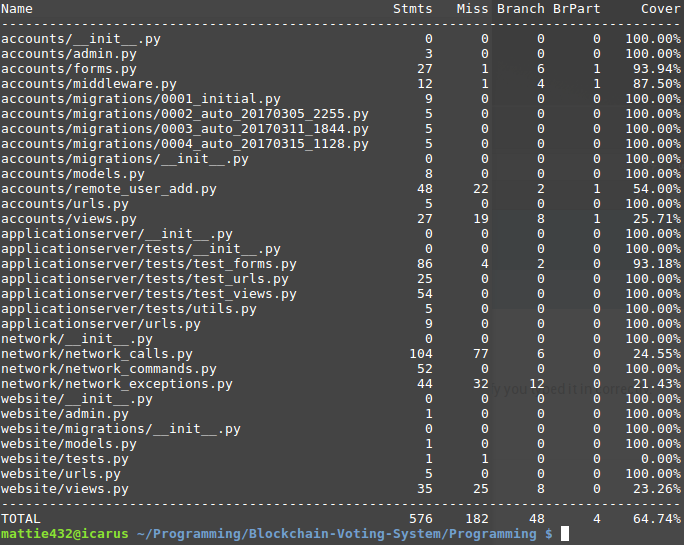
\includegraphics[width=1\textwidth]{code_coverage}}%
	\caption{Test coverage results from the ``Application Server''}
\end{figure}

\subsubsection{Pylint}
Pylint is a Python tool that checks a module for coding standards with a range of checks run from Python errors, missing docstrings, unused imports, unintended redefinition of built-ins, to bad naming and more. By default Pylint offers an overwhelming amount of information \& errors relating to extremely minor, often stylistic, differences (e.g. \textit{W:675, 0: Class has no \_\_init\_\_ method (no-init)}). This error is not only unuseful, it masks any potential larger problems due to the scale of output Pylint produces (initially for my project over 5,000 lines). To make Pylint more usable I had to configure Pylint to only check areas I specified, this included only displaying detected Errors (rather than information \& warnings) along with certain warnings which I switched on (such as `too many arguments'). I started with a very basic configuration and steadily increased it over the duration of my project. 



\cleardoublepage
\subsection{Ethereum}
\subsubsection{What is Ethereum}
In summary, Ethereum is an open software platform based on blockchain technology that enables developers to build and deploy decentralized applications. The block chain is a decentralized network of computers who, at the most basic level, all maintain a ledger in consensus with each other. One block is added at a time, each block contains a mathematical proof that verifies it's addition to the chain and the transactions within are protected by a strong cryptography.
 
Ethereum is poised to become the next greatest innovation based on block chain technology so is Ethereum similar to Bitcoin? The answer is sort of, but not really. Like Bitcoin, Ethereum is a distributed public blockchain network, however there are some significant technical differences between the two. The most important distinction to note is that Bitcoin and Ethereum differ substantially in purpose and capability. Bitcoin offers one particular application of blockchain technology, a peer to peer electronic cash system that enables online payments. While the bitcoin blockchain is used to track ownership of digital currency (bitcoins), the Ethereum blockchain focuses on running the programming code of decentralized application \citep{55_what_is_ethereum_a_step-by-step_beginners_guide_2017}.

Ethereum enables developers to build and deploy decentralized applications. A decentralized application or Dapp serves some particular purpose to its users, for example Bitcoin, is a Dapp that provides its users with a peer to peer payment system. Because decentralized applications are made up of code that runs on a blockchain network, they are not controlled by any individual or central entity. Running these Dapps on a decentralized Platform, the blockchain, they benefit from all of its properties \citep{54_ethereum_explained_2017}:

\begin{itemize}
	\item Immutability, a third party cannot make any changes to data.

	\item Corruption \& tamper proof as apps are based on a network formed around the principle of consensus, making censorship impossible.

	\item No central point of failure, as Dapps can be run on every node in the network.

	\item Secured using cryptography, applications are well protected against hacking attacks and fraudulent activities.

	\item Zero downtime, Dapps never go down and can never be switched off.

\end{itemize}

\cleardoublepage
\subsubsection{Ethereum Blockchain}
The concept of the blockchain was originally outlined in a white paper \citep{12_nakamoto_2008} authored under the pseudonym Satoshi Nakamoto in November of 2008 and was quickly followed by an open source release of the Bitcoin proof-of-concept source code in January 2009 \citep{13_nakamoto_2009}. This is the distributed ledger which underpins the entirety of the Bitcoin and Ethereum systems. A distributed ledger is a consensus of replicated, shared, and synchronized digital data geographically spread across multiple sites, countries, and/or institutions \citep{24_distributed_ledgers_and_blockchain_technology_2016}. This ledger is stored locally on every node in the network which is running the full version of the blockchain software \citep{14_bitcoin_2009} and records every transaction sent and confirmed on the network (the current size of the Ethereum Blockchain is around 21GB, March 2017\citep{25_blockchain_size_2016}). This complete history, coupled with the fact that it is an open network means that anyone can see what is happening in the network, not just now but during all periods in the past. This is extremely powerful as it allows an individual to fully audit the entire contents of the Blockchain without relying on external parties. This process is, in fact, what happens when you first download the full version of many blockchain reliant software \citep{20_developer_guide_bitcoin_2016}.

While the Ethereum Blockchain is not the only most mature distributed ledger in existence, it does have several years of being a publicly proven method to achieve distributed consensus and does this via the `proof-of-work mining' process \citep{24_distributed_ledgers_and_blockchain_technology_2016}. This is how new information gets added to the blockchain, by nodes in the network running a special `mining' variant of the Ethereum software which uses considerable computing resources to win the right to add another block to the Blockchain which is accompanied by a reward for the winning user. The concept of `proof-of-work' is a method of ensuring that the information being added to the Blockchain was difficult (in terms of cost and time) to be made, though is easy for others to validate that the requirements were met \citep{26_blockchain_mining_-_distributed_ledgers_and_blockchain_technology_2016}. This means that the expenditure of computing power serves to secure the integrity of the Blockchain, while the miners themselves verify through public-private key cryptography the validity of each transaction they include in a block.

Blocks are chained together making it impossible to modify transactions included in any one block without modifying all following blocks; as a result, the cost to modify a particular block increases with every new block added to the block chain, magnifying the effect of the proof of work \citep{20_developer_guide_bitcoin_2016}\citep{38_proof_of_work_-_masterpage_2016}. This is why, although a transaction is deemed clear upon its inclusion in a block on the Blockchain, best practices dictate that a user considers a transaction confirmed after its inclusion in a block and the addition of five subsequent blocks to the Blockchain \citep{27_confirmation_-_bitcoin_wiki_2016}.

The difficulty of the proof-of-work mining needs to be controlled, so that an average mining time of around 12 seconds per block is maintained. This time is somewhat arbitrary but is an attempt to find a balance between accepting transactions quickly and minimizing instability and waste in the network, as, while a new block is being distributed other miners will be working on an obsolete problem. As more miners join the network the block creation rate will increase due to the greater collective computational power. Therefore, every 2,016 blocks the difficulty of the mathematical challenge is recalculated so that the average mining time returns to normal \citep{20_developer_guide_bitcoin_2016}\citep{26_blockchain_mining_-_distributed_ledgers_and_blockchain_technology_2016}.

Despite the media often suggesting that bitcoin (and the Blockchain technology behind it) is an anonymous payment system, the Blockchain is in fact a transparent record of all user transactions on the network. Blockchain transactions are in fact pseudonymous, and your transactions in the network are like writing under a pseudonym. If an author's identity is ever linked to their pseudonym then everything written under that pseudonym will be revealed \citep{28_anonymity_2016}. This is particularly poignant when considering the Blockchain as every transaction is stored forever, therefore a compromised address could lead to all transactions being linked to a person. There are however ways to reduce the amount of statistical analysis which can be done on transactions that a person is a part of which help to achieve reasonable anonymity.

\subsubsection{Mining \& Ether}
Ether is the fuel of the Ethereum system. It is the currency of the Ethereum network with which the payment of computation is achieved. Ethereum, like all blockchain technologies, uses an incentive-driven model of security where transaction consensus is based on a ``proof-of-work'' criterion of a given difficulty.

The block chain on which the Ethereum executes certain environment is known as the Ethereum Virtual Machine (EVM) \citep{54_ethereum_explained_2017}. Each participating node within the network runs the EVM and performs the proof of work algorithm called Ethash which involves finding a nonce input to the algorithm so that the result is below a certain threshold (depending on the difficulty) \citep{57_introduction_ethereum_frontier_guide_2017}. There is no better strategy to find such a nonce than enumerating the possibilities while verification of a solution is trivial and cheap. If outputs have a uniform distribution, then we can guarantee that on average the time needed to find a nonce depends on the difficulty threshold, making it possible to control the time of finding a new block just by manipulating difficulty \citep{57_introduction_ethereum_frontier_guide_2017}.

This is how transactions are validated, new transactions are forwarded around the network and placed into a pool of unconfirmed transactions. These are not considered `accepted' yet but are available for all to see almost instantaneously. Miners draw from this pool to create a candidate next set of transactions to be officially accepted which will form the next block. The full text of all of these candidate transactions, along with the hash of the previous block and a nonce, are input into the the hash function (Ethash) and miners will try different values for the nonce until the resulting hash is below a certain value. Because it's a cryptographic hash, there's no way to find a nonce that satisfies the output hashes condition other than attempting to guess \citep{20_developer_guide_bitcoin_2016}. At this point, all of the miners are in a competition to find the hash first, each with a potentially different set of transactions to confirm. Once a miner succeeds they announce their solution to the rest of the network, their block becomes the next block in the Blockchain, and the transactions therein become confirmed. This strategy means that one miner will choose the next set of confirmed transactions, but the hash function effectively makes the miner a random one. All other mines then validate this new block, and the transactions held within, and can choose to accept it and start work on the next block. As the new block contains the hash of the previous block, this forms a chain of confirmed blocks securing the order of the transactions held within.

Occasionally, two miners may find a solution to the problem at the same time creating two potential next blocks in the chain. When miners produce simultaneous blocks at the end of the block chain, each node individually chooses which block to accept, this is usually the first block they see. Eventually another miner finds the solution to another block which attaches to only one of the competing blocks. This makes that side of the fork stronger and, as the general consensus is to use the strongest chain, other nodes will switch to this longer Blockchain \citep{20_developer_guide_bitcoin_2016}. While this is statistically unlikely to happen, it is even more unlikely for the subsequent blocks to be solved at the same time, meaning that one fork will grow quicker than the other and the fork will resolve itself quickly. Transactions that were in the fork that wasn't chosen are not lost and are placed back into the unconfirmed transactions pool \citep{4_driscoll_2016}. The fact that the end of the chain can be forked and rearranged means you shouldn't trust transactions at the end of the chain as much as ones further back. In Ethereum, a transaction is not considered confirmed until it is part of a block in the longest fork, and at least five blocks follow it. In this case we say that the transaction has ``5 confirmations''. This gives the network time to come to an agreed-upon the ordering of the blocks \citep{35_nielsen_2013}.

The successful miner of a block receives a reward for the 'winning' block, consisting of exactly 5.0 Ether along with all of the gas expended within the block, that is, all the gas consumed by the execution of all the transactions in the block. Over time, it's expected the gas reward will dwarf the block reward and become the main incentive for miners to continue working \citep{57_introduction_ethereum_frontier_guide_2017}.

\subsubsection{Transaction Costs \& Gas}
Ethereum does have a small transaction fee, just like Bitcoin, where users pay a relatively small amount to the executor of your transaction. The sender has to pay the fees at each and every step of the activated program, this includes the memory, storage and computation \citep{54_ethereum_explained_2017}. The size of the fee paid is equivalent to the complexity of the transaction, i.e. the more complex the commands you wish to execute, the more gas (and Ether) you have to pay. For example if ``Alice'' wants to send ``Bob'' 1 Ether unit, there would be a total cost of 1.00001 Ether to be paid by Alice. However if A wanted to deploy a contract or run a contract function, there would be more lines of code executable, therefore more energy consumption placed on the distributed Ether network and she would have to pay more than the 1 Gas done in the first transaction \citep{56_ethereum_2017}. Some computational steps cost more than others, either because they are more computationally expensive or because they increase the amount of data that has to be stored in the state. 

Gas is the internal pricing for running a transaction or contract in Ethereum. The gas system is not very different from the use of kilowatts in measuring electricity except that the originator of the transaction sets the price of gas, to which the miner can or not accept \citep{56_ethereum_2017}. Ether and Gas are inversely related say for instance if the Ether price increases, than Gas price should decrease to maintain the concept of real cost \citep{54_ethereum_explained_2017}. With Ethereum there is also a blocksize limit, so the more space your transaction takes up the more you have to pay to get it validated. With Bitcoin miners prioritise transaction with the highest mining fees. The same is true of Ethereum where miners are free to ignore transactions whose gas price limit is too low. 

The reason for the inclusion of a gas price per transaction or contract is to deal with the Turing Complete nature of Ethereum and its EVM essentially to guarantee that code running in the network will terminate. So for example, 0.00001 Ether or 1 Gas can execute a line of code or some command. If there is not enough Ether in the account to perform the transaction or message then it is considered invalid. This aims to stop denial of service attacks from infinite loops, encourage efficiency in the code and make any potential attacker pay for the resources they use (whether that be bandwidth, CPU calculations or storage) \citep{56_ethereum_2017}.

\subsubsection{Smart Contracts}
\label{sec:SmartContracts}
Smart contracts are the key element of Ethereum. In them, any algorithm can be encoded, they can carry arbitrary state and can perform any arbitrary computations even being able to call other smart contracts. This gives the scripting capabilities of Ethereum tremendous flexibility \citep{59_peyrott_senanayaka_2017}. When run a smart contract becomes like a self-operating computer program that automatically executes when specific conditions are met and because they run on the blockchain, they run exactly as programmed without any possibility of censorship, downtime, fraud or third party interference. While all blockchains have the ability to process code, most are severely limited. Ethereum is different in this respect as rather than giving a set of limited operations, Ethereum allows developers to create whatever operations they want allowing developers to build thousands of different applications that go far beyond anything seen previously \citep{55_what_is_ethereum_a_step-by-step_beginners_guide_2017}.

The Ethereum Virtual Machine is where smart contracts are run. It provides a more expressive and complete language than bitcoin for scripting and is Turing Complete. A good metaphor is that the EVM is a distributed global computer where all smart contracts are executed \citep{58_the_hitchhikers_guide_to_smart_contracts_in_ethereum_2017}. There are several higher level languages used to program smart contracts, but Solidity is the most mature and widly adopted. Its syntax is similar to that of JavaScript, its statically typed, supports inheritance, libraries and complex user-defined types among other features.

Smart contracts are run by each node as part of the block creation process and, just like in Bitcoin, this is the moment where transactions actually take place. An important part of how smart contracts work in Ethereum is that they have their own unique address in the blockchain. In other words, contract code is not carried inside each transaction that makes use of it. Instead contracts are ``deployed'' to the blockchain in a special transaction that assigns an address to a contract. This transaction can also run code at the moment of creation. After this initial transaction, the contract becomes forever a part of the blockchain and its address never changes. Whenever a node wants to call any of the methods defined by the contract, it can send a message to the address of the contract, specifying data as input and the method that must be called. The contract will then run as part of the creation of newer blocks up (subject to the gas limit or completion) and can return a value or store data \citep{59_peyrott_senanayaka_2017}.

\subsubsection{Why Choose Ethereum}
Ultimately the decision to use Ethereum for this project was an easy one. Ethereum is not just a digital currency, it is a blockchain based platform with many aspects desirable when designing and creating distributed applications. There simply is no other technology (at the time of writing) that can offer the same level of customization of decentralized programming and has a similarly substantial user base.

I initially investigated using the Bitcoin protocol as a method to store data (votes) immutably and reviewed several papers proposing voting solutions \citep{60_flint_2017}. All of these proposals were however `clunky' in design due to the inescapable fact that that is not what Bitcoin was designed for. Bitcoin was written in a stack based language that isn't Turing Complete as it was designed as a distributed value transfer ledger. 

Ethereum, on the other hand, has contracts written in a Turing Complete Language meaning that anything can be done with it given enough time and enough computing power. This means that Ethereum was built specifically to handle smart contracts over simple currency transactions and although Bitcoin could be built upon to allow the functionality that Ethereum has it would seem unnecessary and be likely cause more problems when programming the application.

Ethereums block confirmation time is also much shorter than Bitcoins. Bitcoin is currently at around 10 minutes whereas Ethereum is around 12 seconds. So consequently, while bitcoin transactions normally take a few minutes to be cleared, Ethereum transactions are cleared almost instantly and at most in a matter of seconds.

The choice to use Solidity as the programming language for my Smart Contracts was mostly governed by maturity. The simple fact is, that there is no other competing languages that have sufficient levels of publicly tested development to justify their use. The closest competitor looks to be Viper \citep{61_ethereum_viper_2017} though this is still in the very early stages of development and lacks many features I would require to be able to use it for this application.
	

\cleardoublepage
\subsection{System Design}
\label{sec:SystemDesign}
There were several points to consider when designing the high level plan of this voting system. The most important of which being the need to ensure separation of a voters account (tied to an individual) and the address they use to vote in the ballot contracts. This directly affected how I designed the system and lead to me splitting the system into distinct sections to take on specific roles; the \textit{Application server} (voter interaction), the \textit{Online Account Verifier} (verify the legitimacy of an account to vote) and the \textit{Online Ballot Regulator} (manages the ballot contracts).

\begin{figure}[h]
	\noindent
  	\makebox[\textwidth]{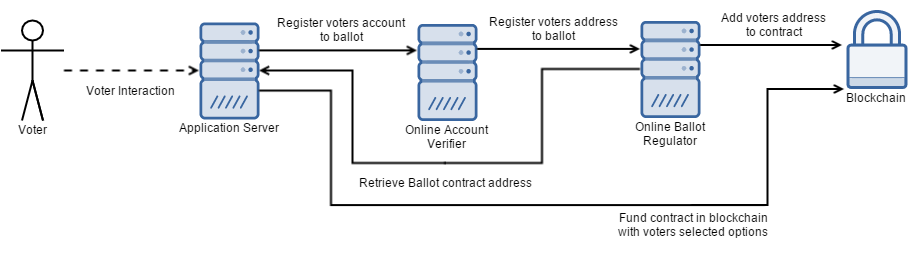
\includegraphics[width=0.8\paperwidth]{blockchain_high_level_overview}}%
	\caption{Outline of system showing the basic interactions between nodes.}
\end{figure}

Splitting the system like this adds both a layer of security and increased scalability. AS all of the data is not centralized on one node (or in one database) this would make it more difficult for a potential attacker to breach the system as they would have to get past the security of at least two nodes to obtain anything useful. The big benefit here is scalability, as if this was scaled up to a general election, more traffic would be seen on some nodes than others (e.g. more logins through the \textit{Application Server} than ballot queries in the \textit{Ballot Regulator}). We could then independently scale each node accordingly.

As each of these nodes are effectively self contained, they only need to expose a select number of services to allow inter-node further decreasing the possibilities for attack. As many of these services only need to be called from other nodes, we can add authentication to these connections to ensure that is upheld. In fact, there are only two external points of contact with this system, the web interface for the voter to use and the blockchain interface to contact other Ethereum nodes, meaning we could black box our system from the outside world fairly completely (see \hyperref[sec:InternalNodeNetworking]{Internal node networking \ref*{sec:InternalNodeNetworking}} sections).

Finally, I chose python as the main language for this system as it has strong frameworks for building web applications (Django) which I heavily utilized these for the \textit{Application Server} \& \textit{External Voter Registration} nodes. There is also strong development of Web3.py \citep{62_pipermerriam_web3.py_2017} which is a python implementation of web3.js, heavily used when interacting with Ethereum through the Geth client. I also discovered the Twisted python networking package \citep{63_twisted_2017} which includes an Asynchronous Messaging Protocol (AMP) implementation for calling remote methods and the Pycrypto library which allowed me to perform the RSA blind signature verification which is crucial to separating a user from their Ethereum address.

\subsubsection{External Voter Registration}
The ``External Voter Registration'' node is meant to represent \textit{some external registrar} who is not directly a part of the designed voting system, but plays a crucial role in the verification of a voters validity (e.g. the UK governments register to vote system). Their role should be purely during the ``pre-election registration'' stage where the voting populous registers their intent to vote in the upcoming election. 

I envision this as being very similar to registering to vote with GOV.UK, where you send your uniquely identifying information (e.g. date of birth, national insurance number, etc) and are then, if verified as a valid voter, registered for the appropriate ballots for your area. As such there would be no need to write this application from scratch as i would make sense to utilize the existing verification systems already in place and modify them to interact with the Ethereum voting system as appropriate. 

For the purpose of demonstrating my application I have written the software for the ``pre-election registration'' node so that I can register a new voter in the system easily (as there needs to be multiple database entries created) and so I can easily deploy a new ballot contract to the blockchain from a specific Ethereum address (necessary so that we have permission to register a voter to a ballot contract). The ``External Voter Registration'' application runs on a Django base, this is because I needed to present a web interface for interaction when registering a new ballot \& user.

\subsubsection{Application Server}
The ``Application Server'' node is the main place for voter interaction with the system. Here, the Django backend provides the web interface for users to log in, register to a ballot \& ultimately vote.

User interaction is centred around a dashboard page which displays core system information to the user (ballots they are eligible for, whether they have voted, etc). From here the user can invoke all voting operations available to them such as registering for a ballot \& voting, to account management options such as changing passwords. When displaying the voting page after a user requests to vote in a ballot, the application server will query the blockchain contract for the voting options \& also display current statistics about the ballot (such as number of registered voters, the current votes per candidate \& voter turnout).

\subsubsection{Online Account Verifier}
The ``Online Account Verifier'' holds the role of authenticating that a user is eligible for a ballot while retaining the anonymity of the final Ethereum address the user casts their vote with. This is accomplished with the use of blind token signing, the process of signing a message without seeing the contents. This means we can verify a voter and return them a signed token which can be sent in future along with an Ethereum address to verify that the address is legitimate. 

\begin{figure}[h]
	\noindent
	
	\begin{center}
	
	Database table holding token requests.
	\end{center}

  	
  	\makebox[\textwidth]{
  	    \begin{tabular}{ | l | p{5cm} | l | l | p{2,5cm} |}
    		\hline
    		token\_request\_id & blind\_token\_hash & user\_id & ballot\_id & created\_on  \\ \hline
    		
    		1 & 54baa883f28a768d6bd352d12c730
    		7d1592d394acea4337a018ee2d0f1
    		43642a & 68401 & 1234 & 2017-04-08
    		18:08:49.527817 \\ \hline
    		
    		2 & 4451458fe4d479387fdca5dde405a
    		16fd2fca2c4f92c516fea78b2f0d27
    		27f7c & 67173 & 1234 & 2017-04-08
    		18:27:25.984678 \\ \hline
    		   		
    		
    	\end{tabular}
  	}%
    	
	\begin{center}
		\hfill \break
		Database table holding token registrations.
	\end{center}


  	\makebox[\textwidth]{
  	    \begin{tabular}{ | l | p{5cm} | p{4cm} | l | p{2.5cm} |}
    		\hline
    		register\_vote\_id & signed\_token\_hash & voter\_address & ballot\_id & created\_on  \\ \hline
    		
    		1 & 19a91bc3d91b5873e5b0e4687a988
    		a08b362bd357a85ce3bc109cba4ed
    		984407 & \href{https://etherscan.io/address/0x79957083494aa13895ae6bad9f04f2bb99f0ad39}{0x79957083494aa13895ae6
    		bad9f04f2bb99f0ad39} & 4321 & 2017-04-08
    		18:30:25.736455 \\ \hline
    		
    		1 & 13jad238sjkgfn39n3asd882nd2d8
    		77ad327dnk3lq9afv4b234akd3nd8
    		98hd82 & \href{https://etherscan.io/address/0x925A8e765F9563D979b576A68210903a9968B8Be}{0x925A8e765F9563D979b5
    		76A68210903a9968B8Be} & 5432 & 2017-04-09
    		12:23:41.162341 \\ \hline
    	\end{tabular}
  	}% 
  	
	\caption{Database table used to store the requests to register an Ethereum address to a ballot for a registered user.}
\end{figure}

The first table is used to verify that a user account has not requested to register for a particular ballot previously with a blind token. The second table is used to keep track of registered Ethereum addresses and which ballot they are registered to. Both of these tables are only used for internal state storage, they are used to determine if a user has already registered for a ballot and show the `register' or `vote' options accordingly. The data stored here is not used by the application server to retrieve any voter credentials. These tables store the token hashes so that we can ensure that tokens cannot be reused by an attacker.

\subsubsection{Online Ballot Regulator}
The ``Online Ballot Regulator'' manages everything to do with the voting ballots. This includes all created ballots in the system and their corresponding Blockchain addresses through to which user accounts are registered to which ballots.

\begin{figure}[h]
	\noindent
		
	\begin{center}
		Database table showing which ballots a userID is allowed to vote in.
	\end{center}

  	\makebox[\textwidth]{
  	    \begin{tabular}{ | l | l | l | l |}
    		\hline
    		ballot\_register\_id & user\_id & ballot\_id & created\_on  \\ \hline
    		
                  1 &    1234 &      1234 & 2017-04-08 18:26:23.440678  \\ \hline
                  2 &    1234 &      6543 & 2017-04-08 18:26:23.440678  \\ \hline
                  3 &    2345 &      6543 & 2017-04-08 18:26:23.440678  \\ \hline
                  4 &   67173 &      1234 & 2017-04-08 18:26:44.067895  \\ \hline
                  5 &   67173 &      4321 & 2017-04-08 18:26:44.134928  \\ \hline

    	\end{tabular}
  	}% 
  	
	\begin{center}
		\hfill \break
		\hfill \break
		Database table holding information about each ballot in the system.
	\end{center}

  	
  	\makebox[\textwidth]{
  	    \begin{tabular}{ | l | p{4cm} | p{4cm} | p{2.5cm} | p{2.5cm} | l |}
    		\hline
    		ballot\_id & ballot\_name & ballot\_address & created\_on & ballot\_interface & ballot\_end\_date \\ \hline
    		
    		1234 & Election of the Member of Parliament for the Harborne Constituency & \href{https://etherscan.io/address/0x127c73af1f9e0eff8226db6bdf04310fdee674f6}{0x127c73Af1F9E0efF8226
    		Db6bdf04310fDEe674F6} & 2017-04-08 18:26:23.440678 & x800358071002e &      1603238400\\ \hline
    		
    		4321 & Election of Police and Crime Commissioner for Edgbaston area & \href{https://etherscan.io/address/0x8C872c720DF854a058C3D1DD54e4CEE51d798B6A}{0x8C872c720DF854a058C3
    		D1DD54e4CEE51d798B6A} & 2017-04-08 18:26:23.440678 & x800358071002e & 1603238400\\ \hline
    		
    		6543 & Referendum on the United Kingdoms membership of the European Union & \href{https://etherscan.io/address/0x7654EC4067e8fA04184D68fF08169A29A3B20F19}{0x7654EC4067e8fA04184D
    		68fF08169A29A3B20F19} & 2017-04-08 18:26:23.440678 & x800358071002e & 1603238400  \\ \hline 		
    		
    	\end{tabular}
  	}%
    
	\caption{Database table used to store the requests to register an Ethereum address to a ballot for a registered user.}
\end{figure}

The ``Online Ballot Regulator'' is where the ``External Voter Registrar'' sends the available ballots for a user account to be stored. This node is the most queried in the entire system as it holds information about ballots the user account is tied to along with the address of ballots in the blockchain.

\subsubsection{Blockchain Ballot Contract}
\label{sec:BlockchainBallotContract}
At the heart of this system is an Ethereum Smart Contract, this is the core from which the entire system design is centred around. The smart contract is how we interact with \& store data in the blockchain \& due to its turing complete programming language we are able to express complex properties which are guaranteed to be upheld. A more detailed explanation of the inner working of smart contracts can be found in the \hyperref[sec:SmartContracts]{Ethereum Smart Contracts \ref*{sec:SmartContracts}} section.

For this Ethereum voting system I have designed a single smart contract that can be modified for each ballot that the system uses. This contract, upon creation, allows a ballot name \& set of candidates to be added so it is re-usable for any number of ballots (note that this still creates distinct \& unique contracts in the blockchain, but their underlying code \& available functions will be the same). I believe that this contract would be suitable for the majority of ballots currently in use however, if the need arose to write different types of ballot contract (maybe a ballot where you can give candidates a percentage of your vote), these could be easily integrated into the system. The full code for the ballot is available in the ``Online Ballot Regulator'' node at \href{https://github.com/Mattie432/Blockchain-Voting-System/blob/master/Programming/4_OnlineBallotRegulator/ethereum/ETHVoteBallot.sol}{ethereum/ETHVoteBallot.sol} which was written in the Solidity smart contract language and a description of the systems steps for deploying a ballot contract is available in the \hyperref[sec:CreatingANewBallotContract]{Ballot Creation \ref*{sec:CreatingANewBallotContract}} section. 

The smart contract is broken down into four distinct sections, the first of which is the global settings \& contract constructor. The constructor is called only on the initial deployment transaction when the contract is first entered into the blockchain. Inside the constructor we set the ballots name \& end date (this is in seconds since epoch) both of which are no longer editable after this point. The constructor also sets the `owner' variable of the contract to the Ethereum address that funds the deploy transaction (in our system this address is under the control of the ``Ballot Regulator'') this owner variable will be used to limit the access to some internal functions further into the contract.

\begin{lstlisting}[caption=Contract constructor called when deploying the contract.]
// ~~~~~~~~~~~~~~~~~~ Contract Constructor ~~~~~~~~~~~~~~~~~~~~~ //
address owner;                // The address of the owner. 
bool    optionsFinalized;     // If we can still add voting options
string  ballotName;           // The ballot name.
uint    registeredVoterCount; // Count of registered addresses.
uint    ballotEndTime;        // seconds since 1970-01-01

// Modifier to only allow the owner to call a function.
modifier onlyOwner {
    if( msg.sender != owner ) throw; _;
}

// This function is called *once* at first initialization into the blockchain.
function ETHVoteBallot(string _ballotName, uint _ballotEndTime)
{
    if( now > _ballotEndTime)
        throw;

    // Set the owner to the address creating the contract.
    owner = msg.sender;
    optionsFinalized = false; 
    ballotName = _ballotName;
    registeredVoterCount = 0;
    ballotEndTime = _ballotEndTime;
}
\end{lstlisting}

\cleardoublepage
The next section sets the ballot options for the contract. First we define a structure for each voting option containing the candidate name \& their vote tally, these are stored in a dynamically sized array called \textit{votingOptions}. The \textit{addVotingOption} function is used to add new candidates to the contract, note the use of `throw' here will terminate the contracts running and refund spent ether. The final function, \textit{finalizeVotingOptions}, sets an internal flag which stops any further modifications to the contracts candidates \& opens up voting to those addresses added to the contract. We have added a modifier to these functions, \textit{onlyOwner} (defined above), which will only allow the address which created the contract to call these functions.


\begin{lstlisting}[caption=Functions used for modifying the ballot during setup.]
// ~~~~~~~~~~~~~~~~~~~~~~~ Ballot Options ~~~~~~~~~~~~~~~~~~~~~~ //
// Structure which represents a single voting option for this ballot.
struct VotingOption
{
    string name;    // Name of this voting option
    uint voteCount; // Number of accumulated votes.
}

// dynamically sized array of 'VotingOptions'
VotingOption[] public votingOptions;

/*
*  Add a new voting option for this ballot.
*  NOTE: this can only be called by the ballot owner.
*/
function addVotingOption(string _votingOptionName) onlyOwner
{
    if( now > ballotEndTime) throw;
    // Check we are allowed to add options.
    if(optionsFinalized == true)    
        throw;

    votingOptions.push(VotingOption({
        name: _votingOptionName,
        voteCount: 0
    }));
}

/*
*  Call this once all options have been added, this will stop further changes and allow votes to be cast.
*  NOTE: this can only be called by the ballot owner.
*/
function finalizeVotingOptions() onlyOwner
{
    if(now > ballotEndTime) throw;

    if(votingOptions.length < 2) throw;

    optionsFinalized = true; // Stop the addition of more options.
}
\end{lstlisting}
\cleardoublepage

The third section refers to `voting options', here we define another structure for voters but rather than use an array we invoke a mapping from the callee address. This means that we can cover the entire address space with the default values of the structure \& only need to change the addresses we wish to give voting eligibility (seen in the \textit{giveRightToVote()} function). The \textit{vote()} method can also be seen which amounts to checking if the voter is eligible \& incrementing the counter of their chosen candidates vote count.

\begin{lstlisting}[caption=Contract code relating to voting.]
// ~~~~~~~~~~~~~~~~~~~~~~~ Voting Options ~~~~~~~~~~~~~~~~~~~~~~ //
// Structure which represents a single voter.
struct Voter {
    bool eligableToVote;    // Is this voter allowed to vote?
    bool voted;             // State of whether this voter has voted.
    uint votedFor;          // Index of 'votingOptions' this voter voted for.
}
// State variable which maps any address to a 'Voter' struct.
mapping(address => Voter) public voters;

/*
*  Allow an address (voter) to vote on this ballot.
*  NOTE: this can only be called by the ballot owner.
*/
function giveRightToVote(address _voter) onlyOwner {
    if(now > ballotEndTime) throw;
    voters[_voter].eligableToVote = true;
    registeredVoterCount += 1;      // Increment registered voters.
}

/*
*  Allow an eligable voter to vote for their chosen votingOption. If they have already voted, then remove their vote from the previous 'votingOption' and assign it to the new one.
*
*  NOTE: if anything fails during this call we will throw and automatically  revert all changes.
*/
function vote(uint _votingOptionIndex) {
    if(now > ballotEndTime) throw;
    if(optionsFinalized == false) throw; //Not finalized, cant vote
    Voter voter = voters[msg.sender];   // Get senders Voter struct

    if(voter.eligableToVote == false) throw;

    // If the voter has already voted then we need to remove their prev vote choice.
    if(voter.voted == true) 
        votingOptions[voter.votedFor].voteCount -= 1;

    voter.voted = true;
    voter.votedFor = _votingOptionIndex;
    votingOptions[_votingOptionIndex].voteCount += 1;
}
\end{lstlisting}

Finally, we include a set of getter functions for various states of the contract. These functions can be used internally by the contract \& called remotely by anyone with the contract address. This is how we allow external verifiability of our ballots.

\begin{lstlisting}[caption=Summary of getter functions.]
// ~~~~~~~~~~~~~~~~~~~~~ Getter Functions ~~~~~~~~~~~~~~~~~~~~~~ //

// Returns the ballots name string.
function getBallotName() returns (string){ ... }

// Returns the number of voting options.
function getVotingOptionsLength() returns (uint) { ... }

// Returns the count of registered voter addresses.
function getRegisteredVoterCount() returns (uint) { ... }

// Returns the name of a voting option at a specific index. Throws if index out of bounds.
function getVotingOptionsName(uint _index) returns (string) { ... }

// Returns the number of votes for a voting option at the specified index. Throws if index out of bounds.
function getVotingOptionsVoteCount(uint _index) returns (uint){...}

// Returns if the voting options have been finalized.
function getOptionsFinalized() returns (bool) { ... }

// Returns the end time of the ballot in seconds since epoch.
function getBallotEndTime() returns (uint) { ... }
    
\end{lstlisting}



\cleardoublepage
\subsection{Pre-election setup}
\subsubsection{Creating a new ballot contract}
\label{sec:CreatingANewBallotContract}
The first thing which needs to be done before any other aspect of the election can take place, is publish the smart contract for each ballot in the election to the blockchain (a deeper analysis of the contract is presented in the \hyperref[sec:BlockchainBallotContract]{Blockchain Ballot Contract \ref*{sec:BlockchainBallotContract}} section). The smart contract I created can be seen as a `template' of sorts, allowing different sets of voting options to be added to a similar core structure. The system requests the `ballot name', `ballots voting options' (provided as a comma separated list) and the `end date' of the ballot. Because all of the Blockchain interactions are handled by the ``Online Ballot Regulator'' we wrap up this information and send it in a network call to the ``Online Ballot Regulator''.

\begin{figure}[h]
	\noindent
	\footnotesize
  	\makebox[\textwidth]{

		\begin{sequencediagram}
			\def\unitfactor{0.65}
			
			
			% External; Voter registration
    		\newthread{EVR}{\shortstack{External Voter \\Registration}}
			
			%Online ballot regulator
			\newinst[5]{OBR}{\shortstack{Online Ballot\\Regulator}}
			
			% Blockchain
    		\newinst[5]{B}{\shortstack{Blockchain \\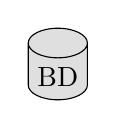
\begin{tikzpicture}[shape aspect=.5]
				\tikzset{every node/.style={cylinder, shape border rotate=90, draw,fill=gray!25}}
			\node  at (1.5,0) {BD};
			\end{tikzpicture}}}{}   
			
			% Display the calls between nodes	
			\begin{sdblock}{Ballot contract registration}{}
				\begin{call}
					{EVR}{\shortstack{Send ballot creation details.\\{[}ballotName, ballotOptions, ballotEndDate{]} }}
					{OBR}{Response {[}Ok{]}}
					
					\begin{call}
						{OBR}{\shortstack{Deploy ballot to the blockchain.\\{[}ballotName, ballotEndDate{]} } }
						{B}{Response {[}ballotAddress{]}}
					\end{call}
					
						\postlevel
					\begin{call}
						{OBR}{\shortstack{Add candidate options to the ballot\\{[}votingOptions{]} } }
						{B}{Response {[}Ok{]}}
					\end{call}
					
					\begin{call}
						{OBR}{\shortstack{Call the contracts finalize method. } }
						{B}{Response {[}Ok{]}}
					\end{call}
					
					\postlevel
					\begin{call}
						{OBR}{\shortstack{Save ballot details to database\\{[}ballotName, ballotAddress{]} } }
						{OBR}{Response {[}Ok{]}}
					\end{call}
				\end{call}
  			\end{sdblock}
  		\end{sequencediagram}
  	
  	}%
	\caption{Registering a new ballot in the blockchain.}
\end{figure}

The \textit{Online Ballot Regulator} does two things, first registering the ballot contract into the Blockchain with the information received from the remote call. This is funded (and therefore deployed) by the \textit{Ballot Regulators} private key and corresponding Ethereum address which, due to the programming of the ballot contract, means that the ballot regulator has exclusive rights to modify the contract. Deploying the contract happens in three stages in the \href{https://github.com/Mattie432/Blockchain-Voting-System/blob/master/Programming/4_OnlineBallotRegulator/ethereum/ethereum.py}{ethereum/ethereum.py} class of the \textit{Ballot Regulator}. First, the contract `template' is deployed to the Blockchain via the Ethereum software run on the server. This is done by sending the compiled contracts bytecode in an Ethereum transaction along with the contract parameters needed to initially setup the contract (the ballot name \& ballot end time). Once the contract is deployed and confirmed into the blockchain we can access the contract at a specific address which we will use from here on out to interact with the contract (e.g. \href{https://etherscan.io/address/0x127c73af1f9e0eff8226db6bdf04310fdee674f6}{0x127c73af1f9e0eff8226db6bdf04310fdee674f6}).

Next we send another transaction for each ballot option, calling an internal method of the contract, to add each of the options to the deployed contract (you can see examples as the 2nd and 3rd transactions in the above link). These options are then immutably added as choices of the ballot.

The final transaction to the contract is to the internal `finalize()' method. After which, no more ballot options can be added and any registered voters are able to cast their votes.

Once the ballot has been deployed to the blockchain the \textit{Ballot Regulator} confirms its validity and then stores internally the ballots name \& Blockchain address. This allows us to query the \textit{Ballot Regulator} later to obtain the correct address for a specific ballot.


\cleardoublepage
\subsubsection{Registering voters in our system}
Once we have a voter who wishes to register, and is eligible to voter in a specific ballot (or set of ballots) we need to add this user to our system so they can log in \& vote.

\begin{figure}[h]
	\noindent
  	\makebox[\textwidth]{

		\begin{sequencediagram}
			
			% External; Voter registration
    		\newthread{EVR}{\shortstack{External Voter \\Registration}}
			
			%Voter
   			\newinst[2]{V}{\shortstack{Voter \\ \\ 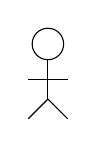
\begin{tikzpicture}
				%\node [fill=gray!20,draw=black,thick ,align=center] {Procesos};
				\draw (0,0) -- (0,0.5); 			%body
    			\draw (-0.25, 0.25) -- (0.25,0.25); 	% arms
    			\draw (0,0) -- (0.25,-0.25); 		% right leg
			    \draw (0,0) -- (-0.25,-0.25);		%left leg
			    \draw (0,0.7) circle(.2); 	% head
			\end{tikzpicture}}}{}

			%Application server
			\newinst[2]{AS}{\shortstack{Application\\Server}}			
			
			%Online account verifier
			%\newinst[1]{OAV}{\shortstack{Online Account\\Verifier}}
			
			%Online ballot regulator
			\newinst[2]{OBR}{\shortstack{Online Ballot\\Regulator}}
			
			% Blockchain
    		%\newinst[1]{B}{\shortstack{Blockchain \\\begin{tikzpicture}[shape aspect=.5]
			%	\tikzset{every node/.style={cylinder, shape border rotate=90, draw,fill=gray!25}}
			%\node  at (1.5,0) {BD};
			%\end{tikzpicture}}}{}   
			
			% Display the calls between nodes	
			\begin{sdblock}{Pre-election registration}{}

				\postlevel
				\postlevel
				\begin{call}
					{V}{\shortstack{Voter registers\\with external\\registrar}}
					{EVR}{\shortstack{Send voter login\\ credentials\\{[}voterID, nonce{]} }}
					
			 	\postlevel
				\begin{call}
					{EVR}{\shortstack{Create login credentials for voter } }
					{AS}{Returned account details{[}voterID, nonce{]}}
				\end{call}
				
				\postlevel
				\postlevel
				\begin{call}
					{EVR}{\shortstack{Inform the verifier of this voter \& their associated ballot(s)\\{[}voterID, ballotID{]} }}
					{OBR}{Ok}
				\end{call}
				
				\postlevel
				\postlevel
				\end{call}
  			\end{sdblock}
  		\end{sequencediagram}
  	
  	}%
	\caption{Sequence diagram showing order of calls when a voter is registered with our system.}
\end{figure}

The first step is validating the user requesting to register is eligible to vote. The validation process is out of the scope of this project but you could imagine this being a similar process to current election registration schemes. Therefore our system has no verification built in and allows anyone to sign up for any ballot of their choosing.

Next we request a new user account is created in the \textit{Application Server} for our voter. A network request is sent and handled by the \href{https://github.com/Mattie432/Blockchain-Voting-System/blob/master/Programming/2_ApplicationServer/accounts/remote_user_add.py}{accounts/remote\_user\_add.py} class which generates a new userID \& random secure password which are then passed back to the caller.

We now register the userID for any ballots they are eligible for. This is done in another network call to the \textit{Online Ballot Regulator} and is handled in the \href{https://github.com/Mattie432/Blockchain-Voting-System/blob/master/Programming/4_OnlineBallotRegulator/onlineballotregulator/network_request.py}{onlineballotregulator/network\_request.py} class. A database entry is created linking the userID to a ballotID  which is used later to verify which ballots a logged in user is eligible for.

Finally the login credentials are sent securely to the user using an applicable method. For a more traditional registration system, this could be sent in the post similar to how you receive a credit card \& pin number (separate letters). It would be possible to encode this information into a QR code format so that the end user need simply scan their received credentials to first log into the system. If the voter validation process was online based, i.e. allowing users to upload their identity documents for automatic processing, we could respond with the users login details almost instantly just like signing up to any secure website (the risks here are reduced as the user is required to change their password on first login anyway).

\begin{figure}[h]
	\noindent
	\vspace{-0.5cm}
  	\makebox[\textwidth]{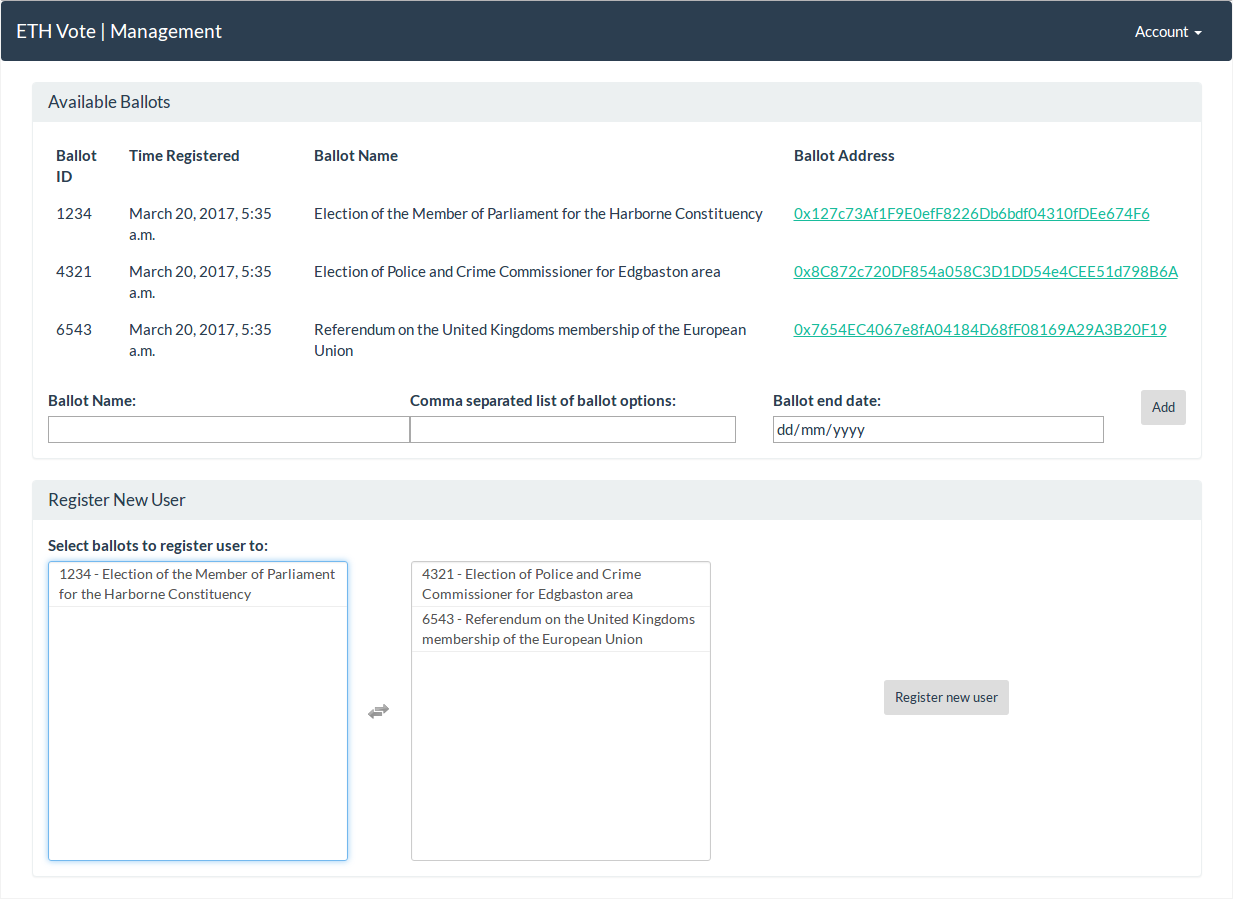
\includegraphics[width=0.62\paperwidth]{external_voter_registration_register_new_user}}%
	\caption{Screenshot of the web interface to the \textit{External Voter Registration} showing the previously created ballots at the top \& the ability to register a new user (to a set of ballots) at the bottom.}
\end{figure}


\cleardoublepage
\subsection{During the Election}
\subsubsection{First login}
Once a user has requested to be registered into the system, and received their initial login credentials, they are able to access the service and log in. Before they are able to access any site content, we enforce a password change and basic user information to be entered. This is for security reasons and is good practice for web applications.

This enforcement is handled by some extra Django middleware in the ``Application Server'' (\href{https://github.com/Mattie432/Blockchain-Voting-System/blob/master/Programming/2_ApplicationServer/accounts/middleware.py}{accounts/middleware.py}) which will not allow access to any internal pages unless the user has already entered their initial information. It does this by checking, before the display of any internal page, if there is a `requires initial information' flag set in the user database and if so refuses to display the requested page and redirects to the initial information request page..

\begin{figure}[h]
	\noindent
	\vspace{-0.25cm}
  	\makebox[\textwidth]{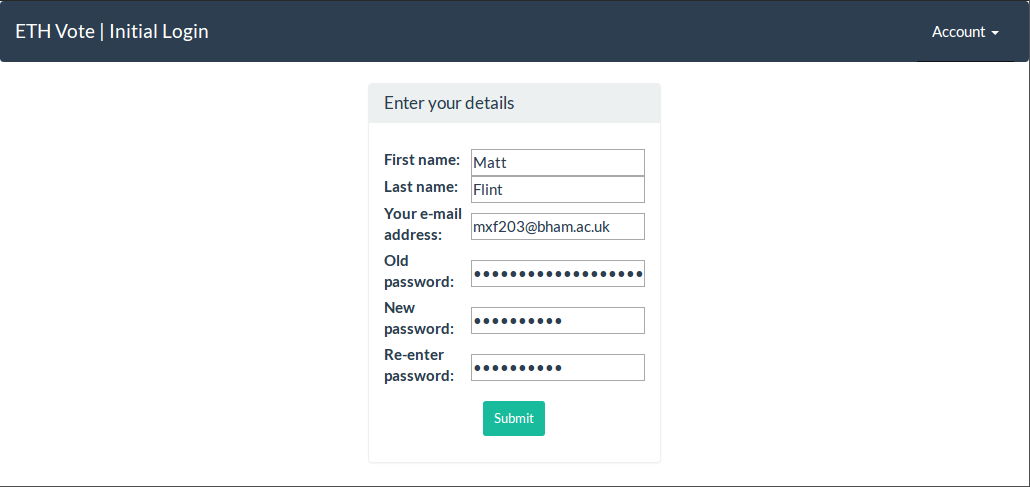
\includegraphics[width=0.8\paperwidth]{application_server_initial_login}}%
	\caption{Initial login information entry page.}
\end{figure}

As the system I produced is only proof-of-concept I have not enforced entry of much information besides an email address and the password reset. If this system was deployed in an actual election you could request for more options to be set here such as contact preferences, display preferences (visually impaired mode) or further security options (maybe setting up two-factor authentication). Once the user has entered the required information they are able to proceed further into the system and access the user dashboard.
 
\cleardoublepage
\subsubsection{Online Registration}
The user dashboard page is the starting place for any user interaction with the system. Here, a list of ballots the user has been approved to vote in is shown along with their corresponding Ethereum address \& associated information such as the current user registration state. Users are presented with a link to an external blockchain viewer showing the transactions of each contract that they can use to independently verify a contracts validity if they wish.

\begin{figure}[h]
	\noindent
	\vspace{-0.25cm}
  	\makebox[\textwidth]{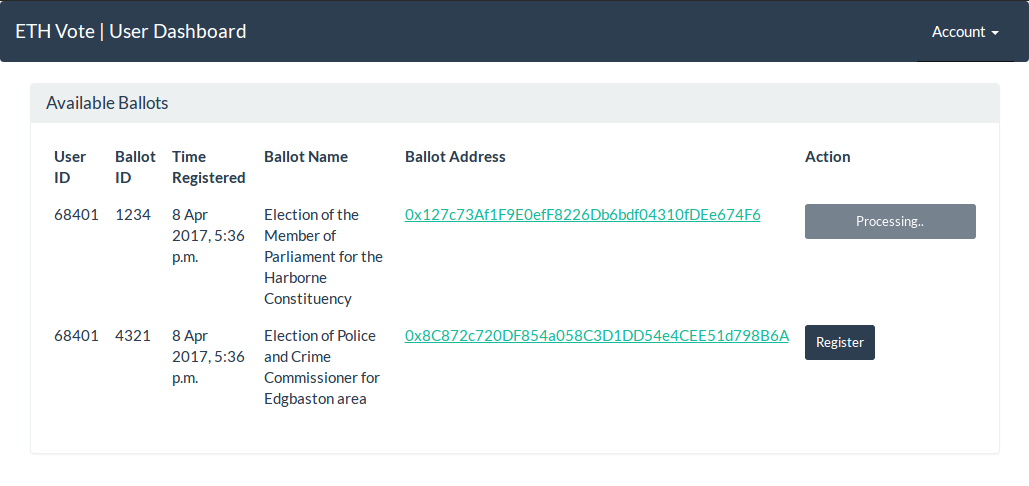
\includegraphics[width=0.8\paperwidth]{application_server_dashboard}}%
	\caption{User dashboard showing ballot information along with the users registration state for each ballot.}
\end{figure}

In order for the user to engage in voting on a ballot we require them to `register' with that ballot. This will start the process of generating a new Ethereum address that will be allowed to interact with the blockchain contract. Note that we could do this automatically without user interaction (possibly after the initial login information has been entered) but I have chosen to offer this as a distinct step which must be invoked in this proof-of-concept system. This is because its easier to demonstrate the separate process of registering a user to a system account to that of registering an address to a deployed ballot contract. In a real world system there would be no need to show this step to the user, as it could cause confusion about what is being registered, and it could easily be abstracted away.

When the user clicks the button to register on a ballot contract we begin the process of generating an Ethereum address for the voter to use, giving it some Ether and allowing it to vote on the selected contract.

\cleardoublepage
\thispagestyle{empty}
\begin{figure}[h]
    \vspace*{-3.8cm}
	\noindent
	\scriptsize
  	\makebox[\textwidth]{

		\begin{sequencediagram}
			\def\unitfactor{0.6}
			
			% External; Voter registration
			%\newthread{EVR}{\shortstack{External Voter \\Registration}}
			
			%Voter
   			\newthread{V}{\shortstack{Voter \\ \\ 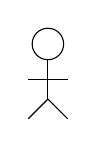
\begin{tikzpicture}
				%\node [fill=gray!20,draw=black,thick ,align=center] {Procesos};
				\draw (0,0) -- (0,0.5); 			%body
    			\draw (-0.25, 0.25) -- (0.25,0.25); 	% arms
    			\draw (0,0) -- (0.25,-0.25); 		% right leg
			    \draw (0,0) -- (-0.25,-0.25);		%left leg
			    \draw (0,0.7) circle(.2); 	% head
			\end{tikzpicture}}}{}

			%Application server
			\newinst[2]{AS}{\shortstack{Application\\Server}}			
			
			%Online account verifier
			\newinst[2]{OAV}{\shortstack{Online Account\\Verifier}}
			
			%Online ballot regulator
			\newinst[2]{OBR}{\shortstack{Online Ballot\\Regulator}}
			
			 Blockchain
    		\newinst[2]{B}{\shortstack{Blockchain \\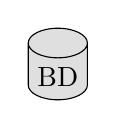
\begin{tikzpicture}[shape aspect=.5]
				\tikzset{every node/.style={cylinder, shape border rotate=90, draw,fill=gray!25}}
			\node  at (1.5,0) {BD};
			\end{tikzpicture}}}{}   
			
			% Display the calls between nodes	
			\begin{sdblock}{Ballot contract registration}{}

				\begin{call}
					{V}{\shortstack{Voter requests to\\vote in a ballot contract}}
					{AS}{\shortstack{Response{[}Ok{]} }}
					
					\begin{call}
						{AS}{Generates a blind token}
						{AS}{{[}blind(T){]}}
					\end{call}					
					
					\postlevel
					\begin{call}
						{AS}{\shortstack{Request token signing\\{[}ballotID, userID, blind(T){]}}}
						{OAV}{\shortstack{Return signed token\\{[}signed\_ballotID(blind(T)){]} }}
						
						\begin{call}
							{OAV}{\shortstack{Check that voterID is\\registered for ballotID\\{[}ballotID, userID{]}}}
							{OBR}{Ok}
						\end{call}							

						\postlevel
						\begin{call}
							{OAV}{\shortstack{Check first time userID\\submits token for ballotID \\{[}ballotID, userID, blind(T){]}}}
							{OAV}{Ok}
						\end{call}		
						
						\postlevel
						\begin{call}
							{OAV}{\shortstack{Signs the token with private\\key associated with the ballotID \\{[}ballotID, blind(T){]}}}
							{OAV}{Ok}
						\end{call}								
						%\prelevel
					\end{call}
					
					\postlevel
					\begin{call}
						{AS}{\shortstack{Extract a signed token from blind token\\{[}signed\_ballotID(blind(T)){]}}}
						{AS}{{[}signed\_ballotID(T){]}}
					\end{call}		
					
					%\postlevel
					\begin{call}
						{AS}{\shortstack{Generate private key \& corresponding Ethereum address}}
						{AS}{{[}privKey, pubKey, voterAddress{]}}
					\end{call}		
					
					\postlevel
					\begin{call}
						{AS}{\shortstack{Register address to vote.\\{[}signed\_ballotID(T), T, voterAddress{]}}}
						{OAV}{Ok}
						
						\begin{call}
							{OAV}{\shortstack{Check token signature is valid.}}
							{OAV}{Ok}
						\end{call}	
						
						\begin{call}
							{OAV}{\shortstack{Check first times seeing this token.}}
							{OAV}{Ok}
						\end{call}	
								
						\postlevel				
						\begin{call}
							{OAV}{\shortstack{Register address to ballot\\{[}voterAddress, ballotID{]}}}
							{OBR}{Ok}
							
							\begin{call}
								{OBR}{\shortstack{Adds voterAddress to ``allowed\\voters'' for the contract\\associated with ballotID}}
								{B}{Ok}
							\end{call}	
							\postlevel
							\begin{call}
								{OBR}{\shortstack{Funds voterAddress with\\enough Ether to cast a vote.}}
								{B}{Ok}
							\end{call}	
														
						%\prelevel
						\end{call}	
													
					%\prelevel
					\end{call}		
					
												
				%\prelevel
				\end{call}
  			\end{sdblock}
  		\end{sequencediagram}
  	}%
  	
    \vspace*{-0.5cm}
	\caption{Sequence diagram showing calls made when a user requests to register with the ballot contract in the blockchain.}
\end{figure}

\cleardoublepage
The process of allowing a voter to interact with a deployed ballot contract is quite involved and is designed to anonymize (to the system and external parties) a voterAddress while still being able to verify that the address is being supplied by a user who is allowed to vote. This verified yet anonymous status is achieved through the use of blind signatures on tokens.

\begin{adjustwidth}{0.5cm}{}
	\paragraph{Blind Signatures}
	\label{sec:BlindSignatures}
	\hfill \break \break

	A ``Blind signature'' is a signing scheme where the signer doesn't know the content of the message he/she is signing but the resulting blind signature can be verified against the original unblinded message just like a regular digital signature \citep{64_ryan_2017}.

	This can be analogized to an individual, Alice, placing a letter inside a carbon paper lined envelope. This is then handed to a trusted third part, Bob, who (without opening the letter) signs the outside of the document \& hands it back to Alice. Due to the carbon paper inside the envelope, Bobs signature is also transferred to the letter within. Alice can then extract the letter which now contains Bobs signature despite him never having seen the letter contents.

	\begin{figure}[h]
	\begin{adjustwidth}{0.5cm}{}
	  	\includegraphics[width=\textwidth]{Blind_Signatures}
		\caption{Blind signature analogy showing how Bob never sees the contents of Alice's message despite being able to sign it.}
	\end{adjustwidth}
	\end{figure}


	Now we can try to translate this to the language of cryptography. Suppose Alice has a message \textit{m} that she wishes to have signed by Bob, and she does not want Bob to learn anything about m. Let \((n,e)\) be Bob's public key and \((n,d)\) be his private key. Alice generates a random value \(r\) such that \(gcd(r, n) = 1\) and sends \(x = (r^e m) \bmod n\) to Bob. The value \(x\) is ``blinded'' by the random value \(r\); hence Bob can derive no useful information from it. Bob returns the signed value \(t = x^d \bmod n\) to Alice. Since \(x^d \equiv (r^e m)^d \equiv rm^d \bmod n\), Alice can obtain the true signature \(s\) of \(m\) by computing \(s = r^{-1} t \bmod n\). Now Alice's message has a signature she could not have obtained on her own \citep{65_bellovin_2015}.
\end{adjustwidth}

I've used the concept of blind signatures in this system to send a randomized Token to the ``Online Account Verifier'' for them to sign. The singing in my system is accomplished using RSA keys and the PyCrypto library \citep{66_pycrypto_the_python_cryptography_toolkit_2017} which abstracts away most of the mathematics and allows the generation of a blind message (see client implementation in ``Application Server'' \href{https://github.com/Mattie432/Blockchain-Voting-System/blob/master/Programming/2_ApplicationServer/user_ballot_registration/views.py#L135}{user\_ballot\_registration/\\views.py} and the corresponding server code at ``Online Account Verifier'' at \href{https://github.com/Mattie432/Blockchain-Voting-System/blob/master/Programming/3_OnlineAccountVerifier/signatures/token_request.py}{signatures/token\_request.py}). The ``Online Account verifier'' has a unique key pair for each ballot that is registered in the system, this means that any tokens signed are valid only as identification for the specific ballot they were requested for.

The order of events for a user to register an Ethereum address to vote is as follows: Firstly, the ``Application Server'' generates a random token to be used in the interaction. This is then blinded with a randomly generated number (as explained in the \hyperref[sec:BlindSignatures]{Blind Signatures \ref*{sec:BlindSignatures}} section) and the public key of the ballot we are requesting to add the address to. Next we send this blinded token across to the ``Online Account Verifier'' to be signed.

When the request to sign the blind token is received by the ``Online Account Verifier'' we initially run a few checks. First, we check to see if the voter requesting to be registered for a ballot is indeed eligible to vote. Secondly, we check that this is the first time we are seeing this user request a token signature for this particular ballot. These checks ensure that users can only register for ballots they are eligible for and each address can only register one address per ballot. If all of our checks pass then we sign this blinded token with the associated ballots private key \& return it to the ``Application Server''.

The ``Application Server'' now has a signed, blinded token (the contents of which have not yet been seen by the ``Online Ballot Regulator'') which we can unblind to reveal a signature of the raw token by the ``Online Ballot Regulator''. We now generate and store an ECDSA keypair \citep{67_kobel_2017} which we can use to derive the Ethereum address the voter will use to interact with the ballot in the Blockchain. The token, token signature \& voterAddress are then sent back to the ``Online Account Verifier'' to be verified before being added to the ballot contract.

This is now the first time the ``Online Account Verifier'' is seeing the token and, as the message is not accompanied by any userID, is unable to link this request to register into the ballot contract to a user. The system can however verify that this request is legitimate by checking the signature of the token against the token, as only a valid voter is able to obtain a signature through the system we can verify that this request is from a genuine voter and should be allowed to proceed. First we check that this is the first time we are seeing this token \& signature (so that the same token cannot be used multiple times) before sending a request to the ``Online Ballot Regulator'' to insert the voterAddress into the ballot contracts list of eligible voters.

As the ``Online Ballot Regulator'' is in control of the Ethereum address that created the ballot contract the node is the only one with the ability to add new voters to the contact (see \hyperref[sec:BlockchainBallotContract]{Blockchain Ballot Contract \ref*{sec:BlockchainBallotContract}} section). We create a new transaction calling the \textit{giveRightToVote()} method of the ballot contract with the voterAddress as a parameter. Once this transaction is confirmed the state change in the ballot contract will mean that, when the voter with the keys to the voterAddress sends a transaction to call the \textit{vote()} method in the ballot, they will be allowed to add their cast vote to the contract. At the same time we also fund the voterAddress with enough Ether to be able to fund their voting transactions (see \href{https://github.com/Mattie432/Blockchain-Voting-System/blob/master/Programming/4_OnlineBallotRegulator/ethereum/ethereum.py#L145}{ethereum/ethereum.py} for the relevant code).

In short, this is how we are able to verify that an Ethereum address is eligible to vote without revealing the user behind the private key.

\cleardoublepage
\subsubsection{Voting}
Once a user has been registered with a deployed ballot contract they are then able to cast their vote into the blockchain. Their registered status will be reflected in the dashboard as the `register' button will change to a `vote' button allowing them to participate in the ballot.

The process of casting a vote is very simple, we call the \textit{vote()} method of the ballot contract with a funded Ethereum transaction \& the voting selection. Because the Ethereum address used to call this method is the one belonging to the user (and has already gone through the `online registration' process) we are allowed to submit our vote to the contract and have it counted.

The process of a user casting a vote in the system is as follows; first, the user selects which ballot they wish to cast a vote in (this is from the set of available ballots shown in the dashboard). The ``Application Server'' sends a network request to the ``Online Ballot Regulator'' requesting the blockchain address for the ballot contract.


\begin{figure}[h]
	\noindent
  	\makebox[\textwidth]{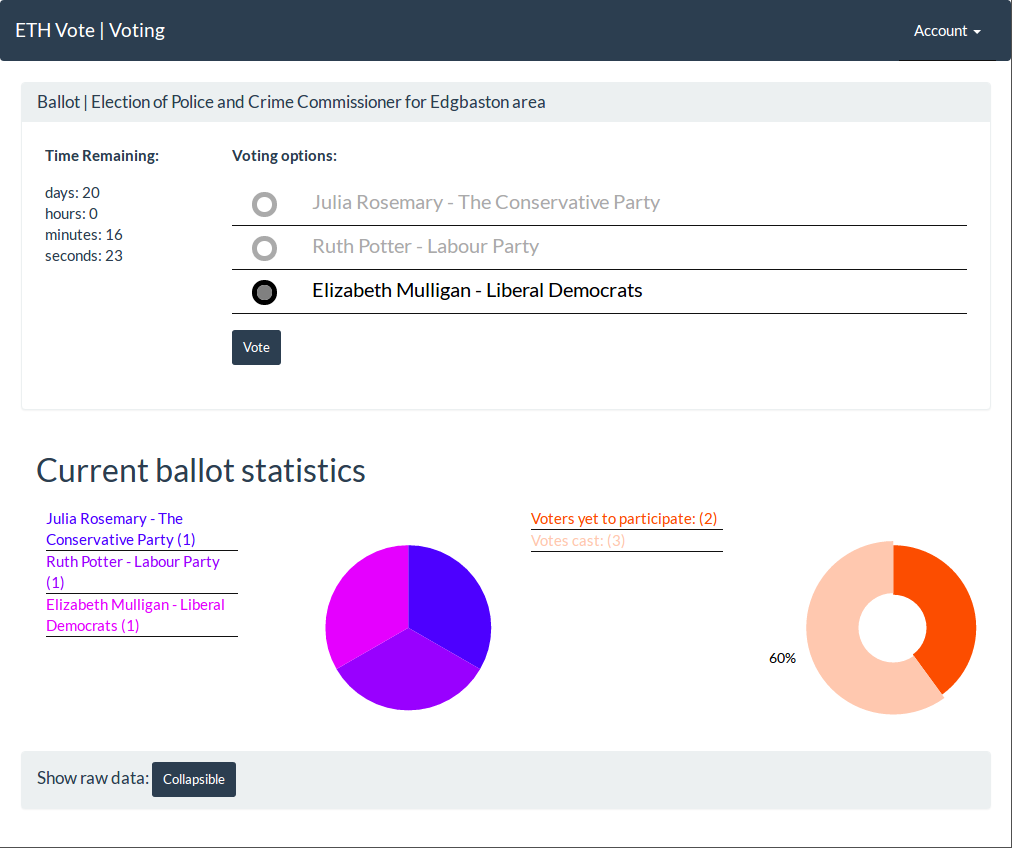
\includegraphics[width=0.6\paperwidth]{vote_ballot}}%
	\caption{Ballot screen presented to the user.}
\end{figure}

From now on all interactions with the contract are handled by the ``Application Server''. As we now have the contract address we can query the blockchain for this contract which returns the contracts definition along with the current `state' of the contract. This means we can retrieve all of the latest information about the ballot directly from the blockchain, information such as `Ballot Name', the list of candidates and the current votes for each candidate. The information available is directly related to the contract design (talked about in \hyperref[sec:BlockchainBallotContract]{Blockchain Ballot Contract \ref*{sec:BlockchainBallotContract}} section) but in my designed system this extends to the current votes for each candidate and the total number of registered voters. This means that we are able to display this information to the user (this can in fact be queried by anyone at any time) and use this to present relevant graphs directly onto the ballot page. At the top of the ballot we present the available candidates, as obtained from the ballot contract, as a radio button selection.

The voter now has all the available information to make their decision, once they wish to cast their vote they choose their voting options and click ``submit''. This generates a Ethereum transaction, funded by the users Ethereum address, which calls the \textit{vote()} function in the ballot contract with the users voting choice as a parameter. The resulting transaction hash acts as a receipt for the voter, allowing them to verify that their vote was successfully accepted and confirmed into the blockchain. This can be done on any blockchain explorer almost instantly due to the propagation properties of the Ethereum network, the system does however provide a link to view the transaction in a trusted explorer for user convenience (e.g. \href{https://etherscan.io/tx/0xd7535e6b492bbcbff7c6b46ea0ce5fd3390071bd01bc9f202e1016486e333cd7}{0xd7535e6b492bbcbff7c6b46ea0ce5fd3390071bd01bc9f202e101648
6e333cd7}).

\begin{figure}[h]
	\noindent
  	\makebox[\textwidth]{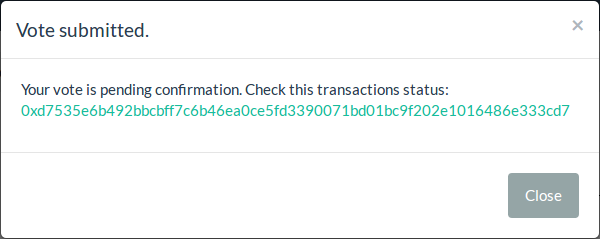
\includegraphics[width=\textwidth]{vote_ballot_submitted}}%
	\caption{Pop-up box on submission of a vote giving the voter the transaction hash.}
\end{figure}

\begin{figure}[h]
	\noindent
  	\makebox[\textwidth]{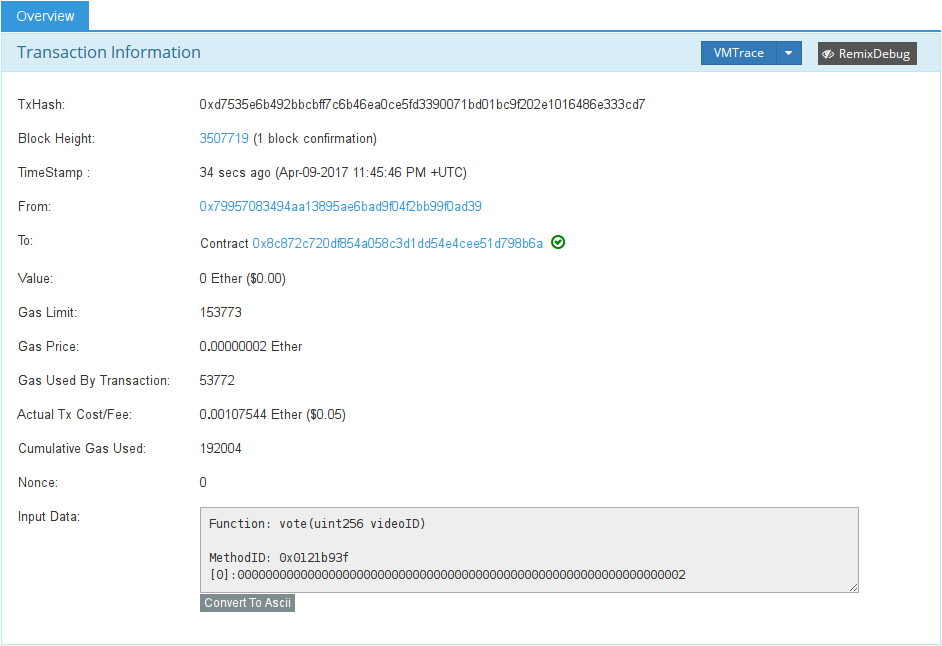
\includegraphics[width=0.85\paperwidth]{vote_ballot_transaction}}%
	\caption{Example of a block explorer showing a confirmed vote transaction.}
\end{figure}

\cleardoublepage

\paragraph{Real time results}
\hfill \break
As discussed in \hyperref[sec:BlockchainBallotContract]{Blockchain Ballot Contract \ref*{sec:BlockchainBallotContract}}, the contract design means that up-to-date election results can be queried from the blockchain contract by anyone at any time. This has huge potential impacts on the way elections could be fought \& would produces a more informed voting populous.

Say, for example, that our our system was opened for voting around the same time as postal votes (assuming that our system is the most common way for people to vote). Candidates would be able to follow the results of their last minute campaign trail, seeing how effective their campaigning was in a certain area by the real time increase in votes.

It also removes a lot of ambiguity around the speculated outcome of the election as the need to rely on opinion polls decreases \& the speculated outcome can be based on `real' votes. This could decrease the likelihood of an election wrongly being declared a `safe outcome' which could potentially cause voters to not worry about submitting their vote (e.g. the results of the UK's EU Referendum \citep{68_curtice_2017}).

\paragraph{Changing a cast vote}
\hfill \break
Another innovation in the way elections could be held is the ability allow voters to change their cast votes in our smart contract. This is, in fact, allowed by my designed ballot contract. A voter can call the \textit{Vote()} method as many times as they like \& if they have previously voted, their vote is removed from the previous tally \& added to the new one.

If deployed for a general election, this would revolutionize the way voters are able to interact with their government. Say for example, if new information relating to a candidate came to light late into the election, voters would not be locked into their uninformed choices. Under the current system, voters who submitted their vote before election day (e.g postal vote) could be misrepresented in their vote for a candidate which they cannot change.

It would also be statistically interesting to be able to analyse the swing of votes as new information came to light. This would be possible as the transaction history of previous votes would still be accessible in the blockchain, therefore we could track how a voter (or more accurately, a voterAddress) changed their opinion over time.

Alternatively this idea could be eliminated completely, we could simply have our ballot contract accept the first vote from each voter as final.

\cleardoublepage
\paragraph{Tentative voting}
\hfill \break
If we were to mix the two innovations outlined above, we could have a brand new kind of election. This would be where voters can post tentative votes, which they reserve the right to change later, but that would allow them to express their opinion for a candidate. This would allow them to see how the general populous feels about a certain ballot without locking them down to that choice.

This would mean that decisions people might not have been willing to stand behind permanently, could be put out tentatively \& then change their minds later based on the sentiments of the public. This ultimately leads to a more informed choice about who has a chance of winning an election, and voters can afford to initially choose candidates based on their merits rather than because they feel they have to vote for someone.

\cleardoublepage
\subsection{Post Election results}
Assuming that you are running a full Ethereum node (that is, have all of the blockchain data available to you) querying any of these getter functions of a ballot contract will not cost you Ether. This is because the state of all of the variables in the contract can be calculated from all of the transactions (which you have locally) therefore the results can be computed without remote calls. The only transactions which you need to pay Ether on are those which perform operations in the blockchain, e.g. saving data or remote computation.

This increases the viability for external parties to audit the ballots in their entirety as if they had an attached cost, due to the size of the election being held, it could have been prohibitively expensive. 

In a general election scenario, public verification would require the publishing of the address of each ballot contract prior to the election beginning. Due to the programming of the contracts this would pose no security risks while increasing transparency during the election. It would also have the benefit of allowing voters to verify that they are interacting with the correct ballot, thus increasing trust throughout the system.

In this scenario I would envisage multiple third parties creating verification systems checking the results of the election in real time through querying these ballot contracts. As the output of the election is now verifiable by anyone, we have fulfilled the ``independent verification of the output'' criterion which we set out to complete.

\begin{figure}[h]
	\noindent
  	\makebox[\textwidth]{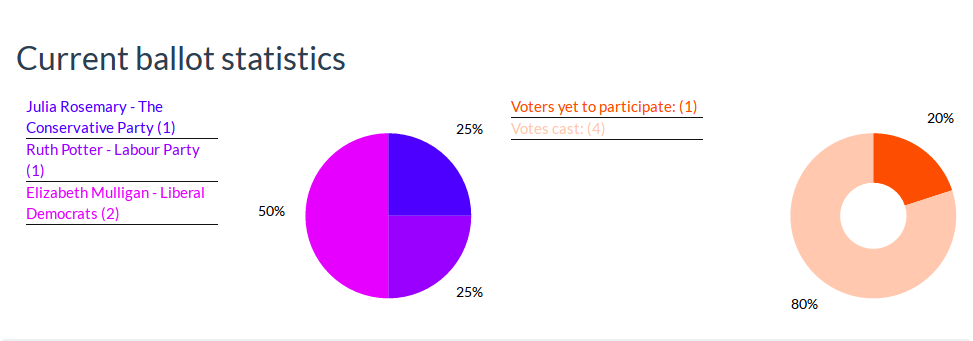
\includegraphics[width=1.2\textwidth]{ballot_results}}%
	\caption{Example of an infographic generated from one ballot deployed to the blockchain.}
\end{figure}



%\printbibliography

\end{document}
